%%
%% Figures for additional distance metric.
%% 

\begin{figure*}
  \centering
  \begin{tabular}{ccc}
    
    \begin{minipage}{2in}
      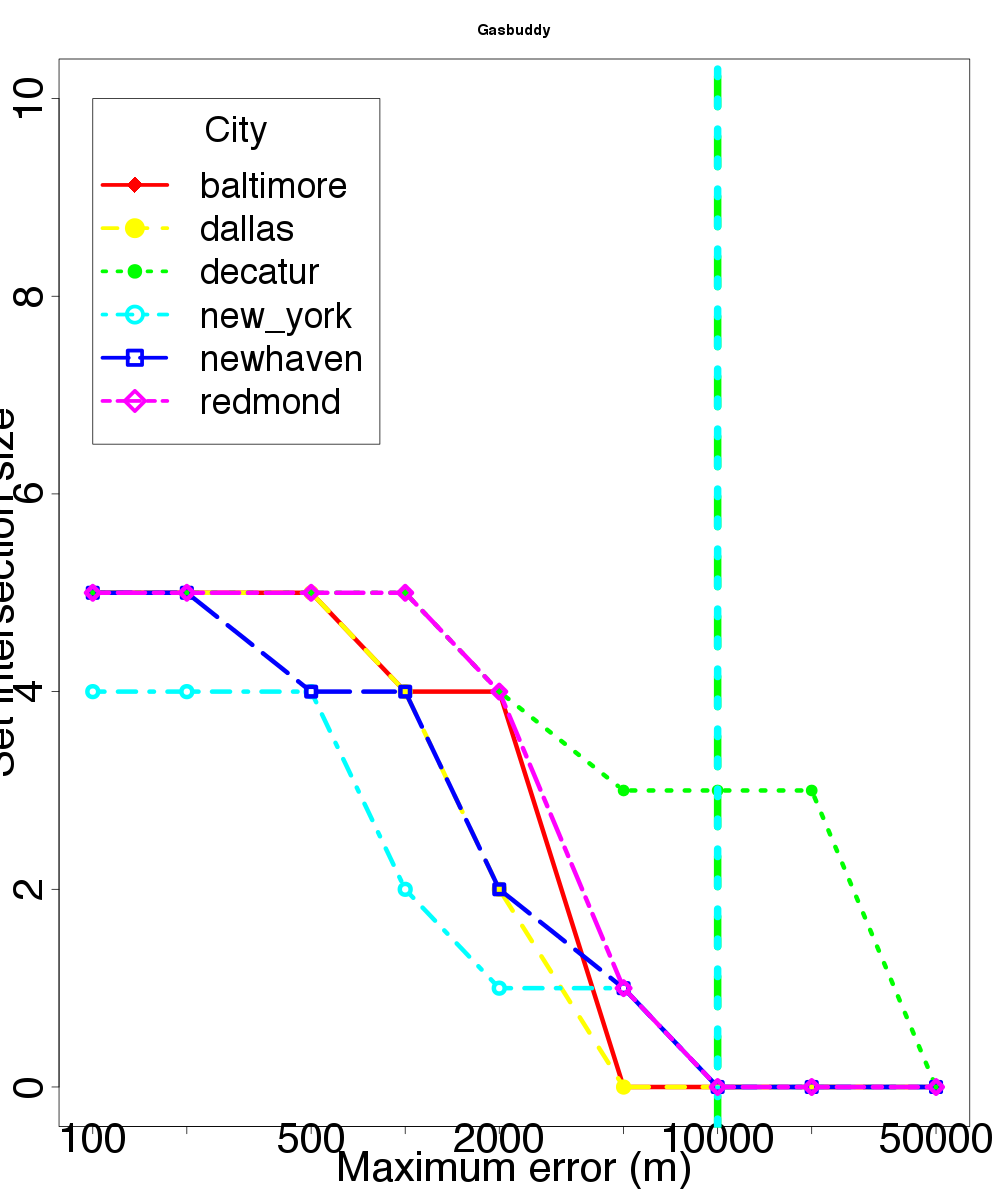
\includegraphics[width=\textwidth]
                      {data/gasbuddy/plots/medians_across_city_si_5}
    \end{minipage}
    
    % [width=.6\textwidth]
    \begin{minipage}{2in}
      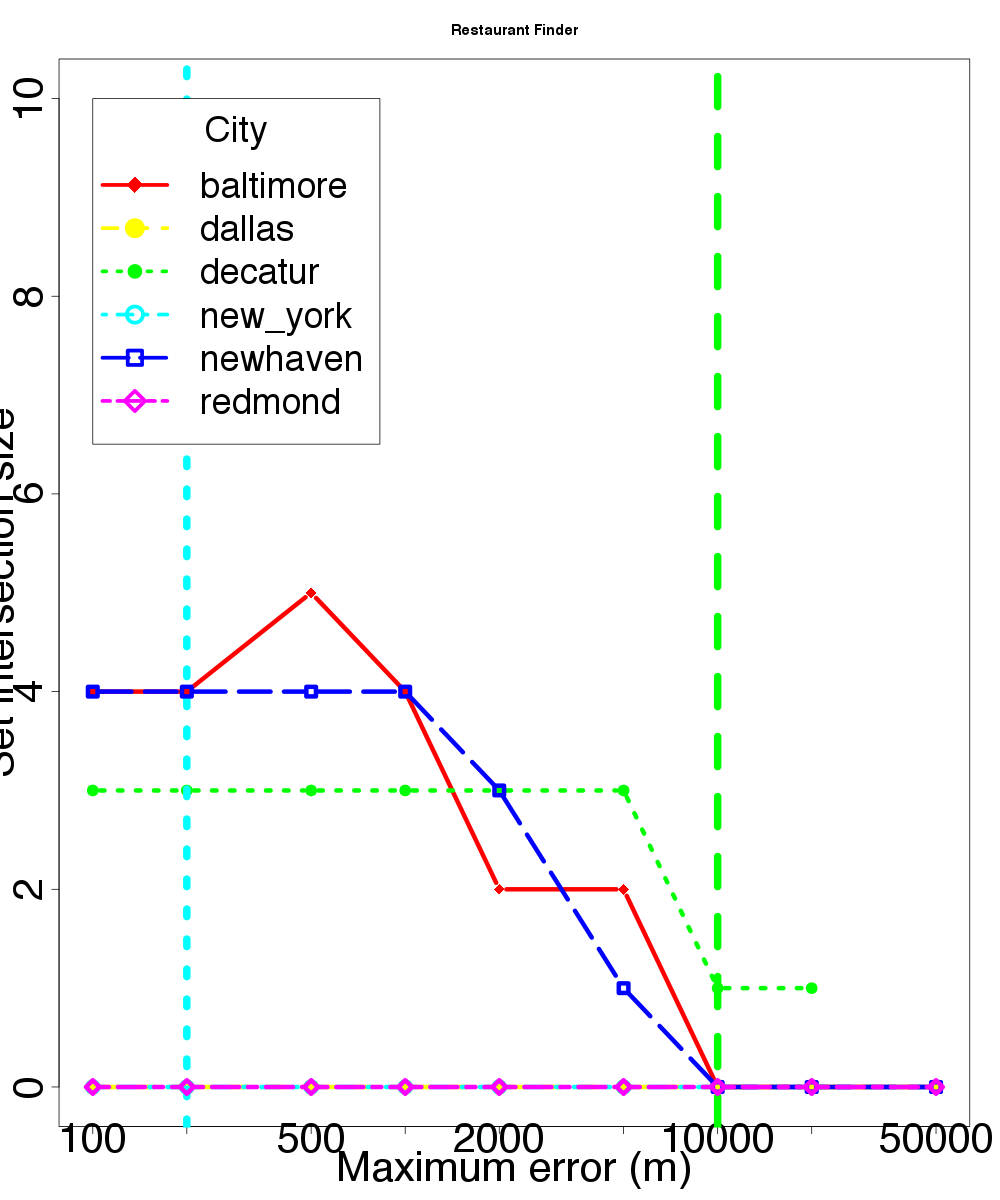
\includegraphics[width=\textwidth]
                      {data/restaurant_finder/plots/medians_across_city_si_5}
    \end{minipage}
    
    \begin{minipage}{2in}
      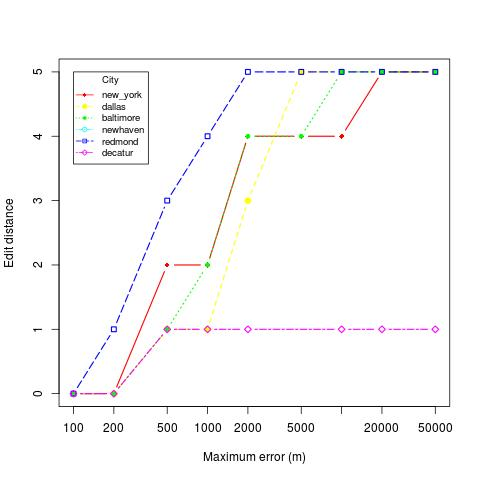
\includegraphics[width=\textwidth]
                      {data/hospitals/medians_across_city_si_5}
    \end{minipage}
    
    \\
    \begin{minipage}{2in}
      
\includegraphics[width=\textwidth]
                      {data/webmd/plots/medians_across_city_si_5}
    \end{minipage}
    
    \begin{minipage}{2in}
      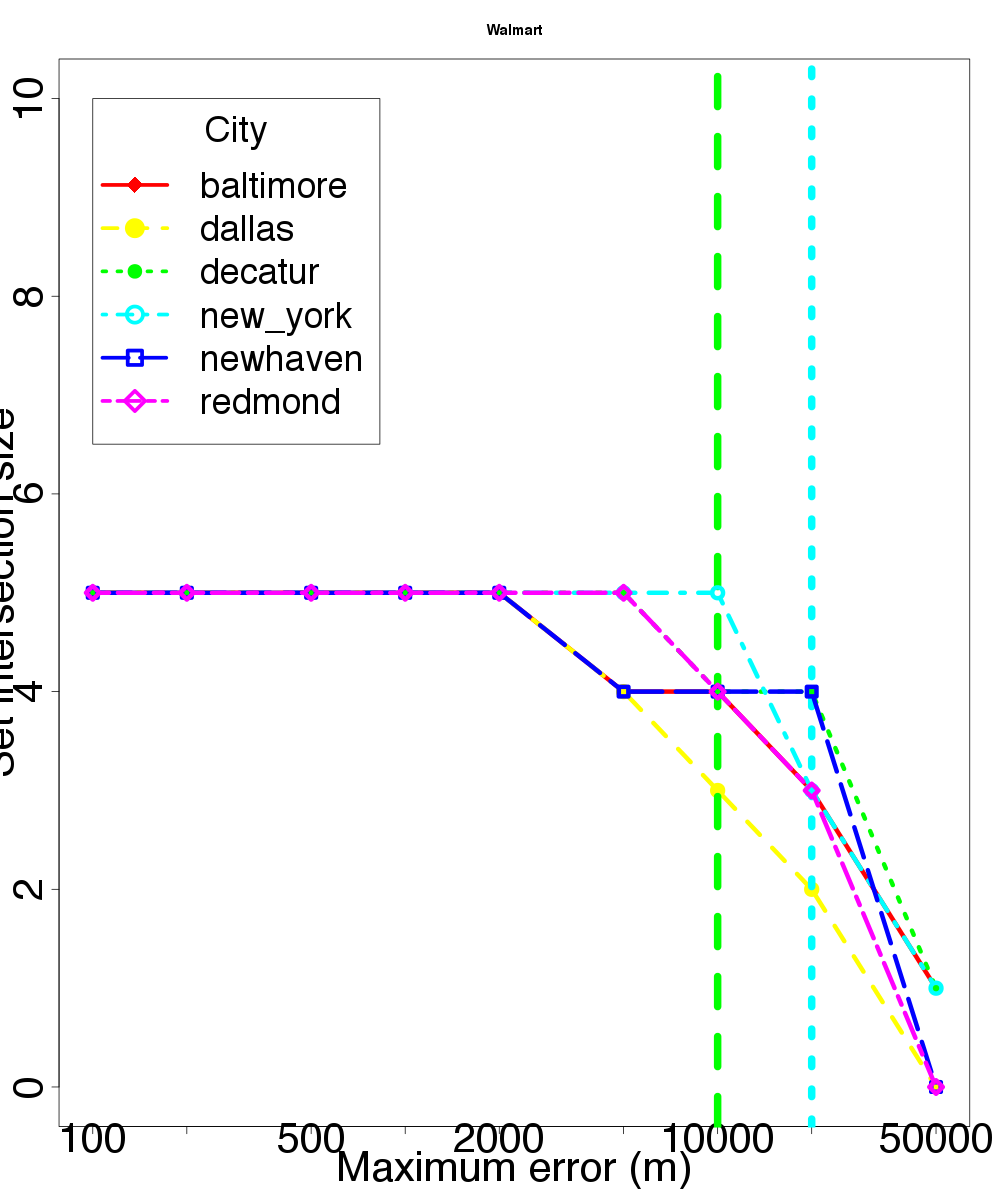
\includegraphics[width=\textwidth]
                      {data/walmart/plots/medians_across_city_si_5}
    \end{minipage}
    
    \begin{minipage}{2in}
      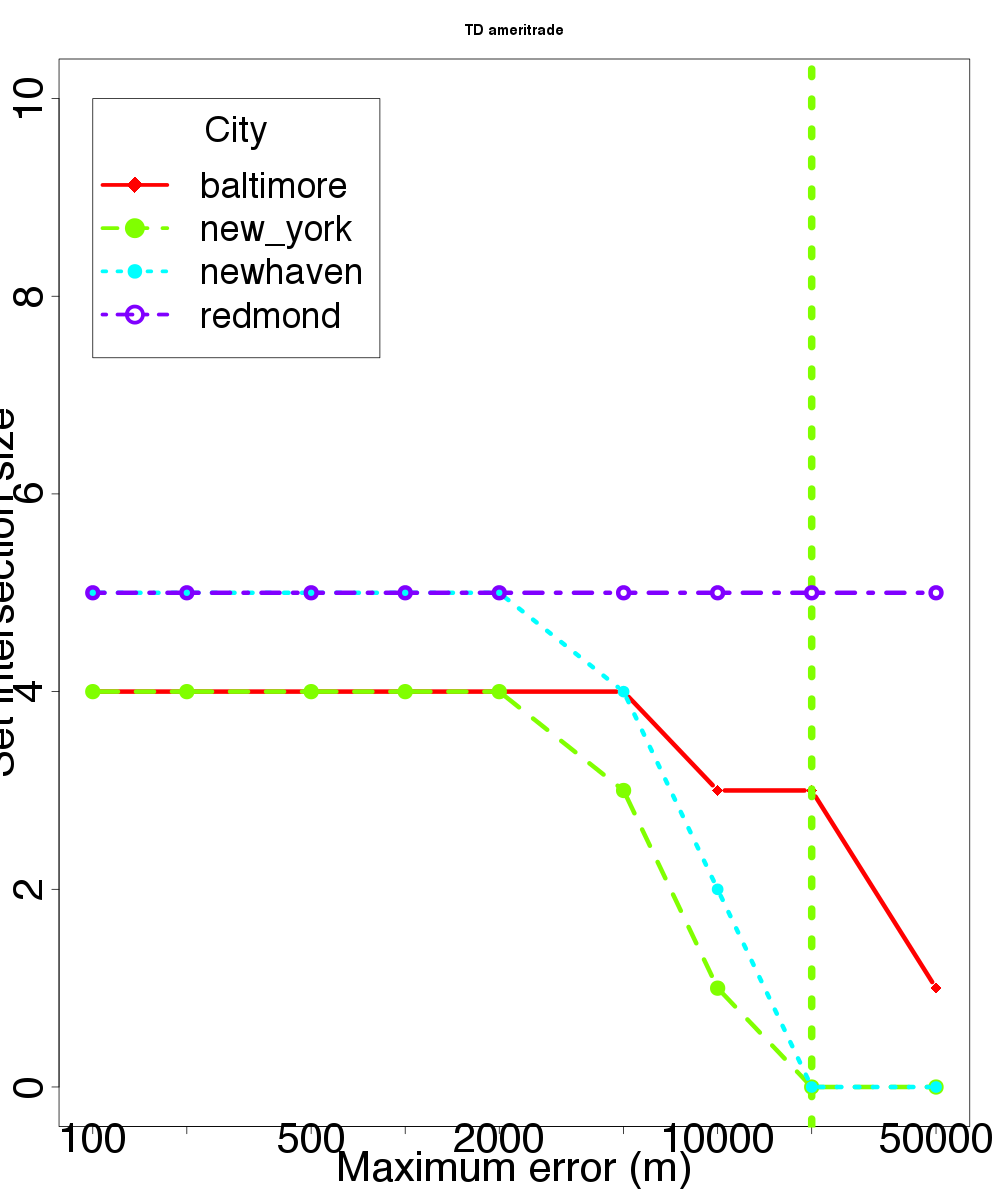
\includegraphics[width=\textwidth]
                      {data/tdbank/plots/medians_across_city_si_5}
    \end{minipage}
  \end{tabular}
  \caption{The set intersection metric considering only the top two
    screens of the app.  The vertical axis indicates the number of
    locations in the nominal output that are also in the reference
    output.}
  \label{fig:set_int}
\end{figure*}
